%%%%%%%%%%%%%%%%%%%%%%%%%%%%%%%%%%%%%%%%%%%%%%%%%%%
%% LaTeX book template                           %%
%% Author:  Amber Jain (http://amberj.devio.us/) %%
%% License: ISC license                          %%
%%%%%%%%%%%%%%%%%%%%%%%%%%%%%%%%%%%%%%%%%%%%%%%%%%%

\documentclass[a4paper,12pt,oneside]{book}
\usepackage[T1]{fontenc}
\usepackage[utf8]{inputenc}
\usepackage{lmodern}
%%%%%%%%%%%%%%%%%%%%%%%%%%%%%%%%%%%%%%%%%%%%%%%%%%%%%%%%%
% Source: http://en.wikibooks.org/wiki/LaTeX/Hyperlinks %
%%%%%%%%%%%%%%%%%%%%%%%%%%%%%%%%%%%%%%%%%%%%%%%%%%%%%%%%%
\usepackage{hyperref}
\usepackage{graphicx}
\usepackage[english]{babel}
\usepackage{titlepic}
\usepackage{wrapfig}

\graphicspath{{./images/}}
\setlength\parindent{0pt}
%%%%%%%%%%%%%%%%%%%%%%%%%%%%%%%%%%%%%%%%%%%%%%%%%%%
% First page of book which contains 'stuff' like: %
%  - Book title, subtitle                         %
%  - Book author name                             %
%%%%%%%%%%%%%%%%%%%%%%%%%%%%%%%%%%%%%%%%%%%%%%%%%%%

% Book's title and subtitle
\title{
	\Huge \textbf{Hybrid rendering}\\
	\huge using Radeon Rays
}
\titlepic{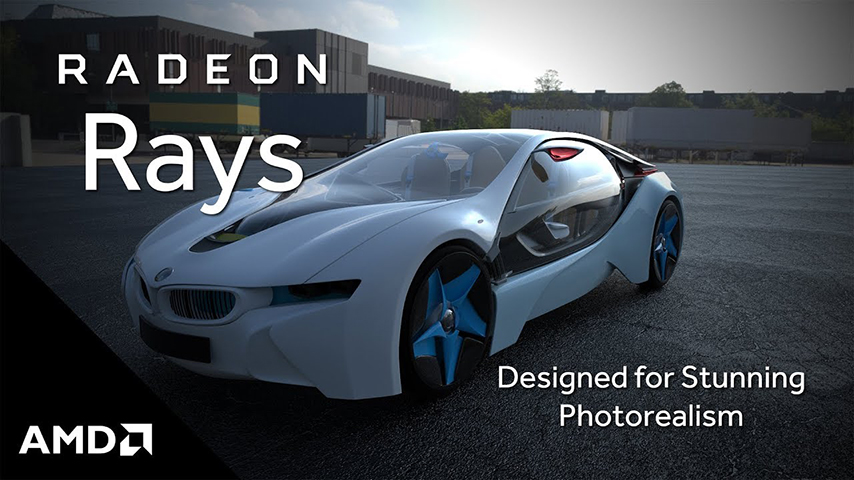
\includegraphics[width=\textwidth]{radeonrays.jpg}}
% Author
\author{
	Stijn Billiet\\\\
	Graduation work 2018-19\\
	Digital Arts And Entertainment\\
	howest.be
}
\date{}


\begin{document}

\frontmatter
\maketitle
\cleardoublepage
%%%%%%%%%%%%%%%%%%%%%%%%%%%%%%%%%%%%%%%%%%%%%%%%%%%%%%%%%%%%%%%%%%%%%%%%
% Auto-generated table of contents, list of figures and list of tables %
%%%%%%%%%%%%%%%%%%%%%%%%%%%%%%%%%%%%%%%%%%%%%%%%%%%%%%%%%%%%%%%%%%%%%%%%
\tableofcontents

\mainmatter
\chapter{Abstract}
This paper was written in an effort to elaborate on hybrid solutions between modern day rasterization engines and powerful ray-tracing ones and to explain rather thoroughly how one could implement this.

TODO methods
TODO results

\chapter{Introduction}
Ray-tracing is usually used in VFX productions to create the most accurate lighting effects, this doesn’t come for free though seeing crisp ray-traced images require countless hours of rendering. With the rise of new ray-tracing capable hardware (e.g. Volta architecture NVIDIA) things are about to change, developers are already putting ray-tracing in some parts of their pipelines, they must however rely on optimization (e.g. De-noising) to keep up with the performance demands. So for the time being we will see a lot of hybrid solutions, but we should see full ray traced engines by the time that our hardware is capable enough.\newline\par

That being said I would like to clarify that rasterization engines aren’t bad, however they are very rough approximations and rely on specific techniques to achieve lighting effects sometimes at the cost of artifacts. We must keep in mind though rasterization engines are here to stay for a while longer due to their immense performance, and not to forget they have been around for a while, their maturity surely pays off seeing what we’ve already achieved with rasterization (e.g. The Witcher 3: Wild Hunt).\newline\par

As the subtitle suggests we will use Radeon Rays for our ray-tracing algorithm, however there are other options out there like Microsoft's DirectX Raytracing. Nevertheless the topics outlined should still hold up when implementing an other API, only the Radeon Rays implementation details would be an exception to that rule. The same essentialy goes for our graphics card specification, OpenGL was used seeing that would be the logical combination, but the information should translate over nicely to other API's. \newline\par

%%%%%%%%%%%%%%%%
% NEW CHAPTER! %
%%%%%%%%%%%%%%%%
\chapter{Research}

This extract should give you a rather thorough overview of the technologies used, however some knowledge regarding graphics programming and/or matrix mathematics is advised.\newline\par

\section{Rendering techniques}
Over the past century many rendering algorithms have been researched/employed. They are all trying to find an answer to the problem of limited rendering capabilities. Seeing that our modern model of light would be completely impractical when it comes to (high speed) simulations, meaning it would take an obscene amount of time to calculate.\newline\par

Therefore people have come up with ways to more efficiently model the phenomenon of light. The most prominent models being: ray tracing (ray casting) and rasterization. The aforementioned models will be covered in the following subsections.

\pagebreak

\subsection{Raytracing}

\begin{figure}[h]
	\caption{Illustration of different ray-casting solutions}
	\centering
	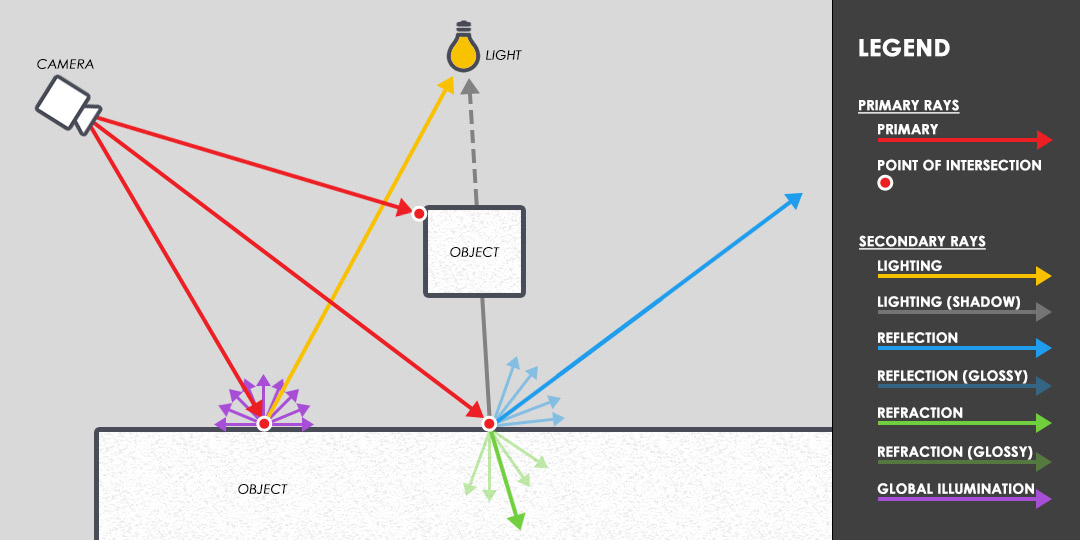
\includegraphics[width=0.95\textwidth]{raycasting.jpg}
\end{figure}
\subsubsection{Definition}
In short ray-tracing is a rendering technique that can produce lifelike lighting effects. A ray-tracing algorithm essentially achieves this by sending out rays for every pixel of our framebuffer (camera) towards the corresponding scene geometry. Based on the technique we can send out additional bounces (secondary rays). It then basically backtracks that chain of light-rays to accumulate material/light information to then calculate the final pixel color.

\subsubsection{Ray casting}

As addressed before ray-tracing essentially probes material and light information through the use of rays. There are 2 sets of rays, we've got primary rays and secondary rays. Primary rays are the first rays being sent out, the rays from camera towards the scene geometry. These primary rays are essentially doing the same as with rasterization in the sense that they only probe at material information. It becomes interesting however when we cast our secondary rays, these secondary rays have their origins at the interception point of the primary rays and the scene geometry. Their direction on the other hand are totally dependent on the technique that is employed, meaning that we will use different techniques to bounce/direct them based on the effect required  (e.g. shadows, reflections, etc.).\newline\par

\pagebreak

\subsection{Rasterization}

\begin{figure}[h]
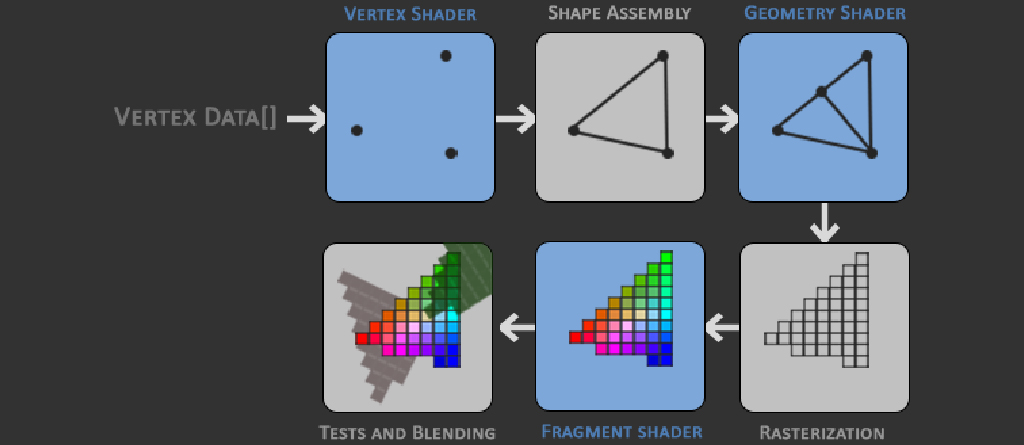
\includegraphics[width=\textwidth]{rasterization.jpg}
\caption{Rasterization graphics pipeline.}
\end{figure}

\subsubsection{Definition}
Rasterization is an algorithm designed to display three-dimensional objects on a two-dimensional screen. It's very fast seeing this algorithm is parallel in nature and can thus make full use of the GPU. The results of rasterization have gotten very good over the years, very convincing at relatively low compute performance. However there are certain limitations to this algorithm, seeing it's main goal is to get graphics in screen space.\newline\par

\subsubsection{Graphics pipeline}
With rasterization objects on screen are created from meshes. A mesh is a collection of three-dimensional points a.k.a. vertices. These vertices are the main resource needed for rendering, these go through what's called the rendering pipeline to then be converted into screen pixels. The rendering pipeline or more formerly known as the graphics pipeline acts as a conceptual model that describes what steps a graphics system needs to performs to be able to render aforementioned meshes to a 2D screen. \newline\par
\pagebreak

\subsubsection{Vertex shader}
\begin{figure}[h]
	\centering
	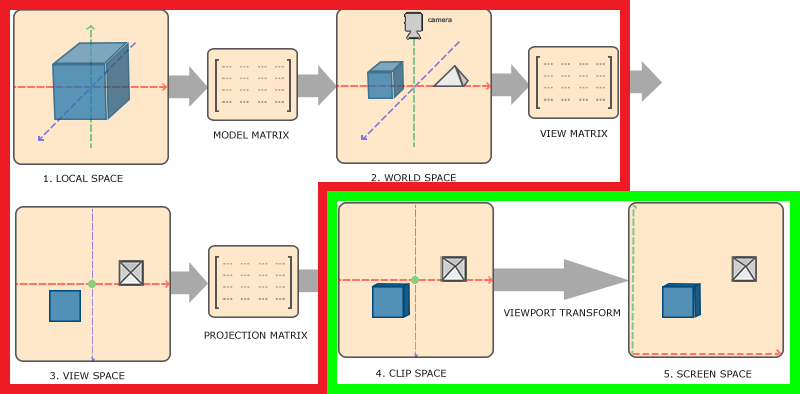
\includegraphics[width=0.8\textwidth]{coordinate_systems.png}
	\caption{Model space to screen space.}
	\label{fig:coordinates}
\end{figure}
The first stage is the vertex shader which essentially transforms the vertices to their correct
positions, the vertices have to be transformed seeing that they are defined in their own local transform space(vertices positions are defined relative to their own center point). The vertices are defined this way as a means to make it easier for modelers, they quite simply have to define the vertices relative to the modeling software's gizmo.

\subsubsection{Shape assembly}
\begin{figure}[h]
	\centering
	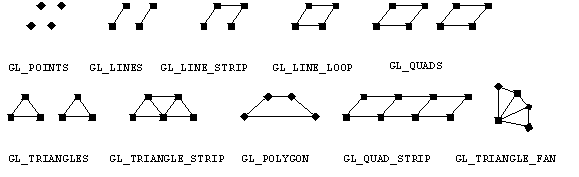
\includegraphics[width=\textwidth]{primitives.png}
	\caption{List of possible OpenGL primitives.}
\end{figure}

The second stage is the shape assembly which is in charge of creating primitives out of these verts. The developers have to specify the wanted primitive (e.g. triangle) the GPU then uses that information to interpret the a collection of vertices as said primitive.\newline\par

\pagebreak

\subsubsection{Geometry shader}
\begin{figure}[h]
	\centering
	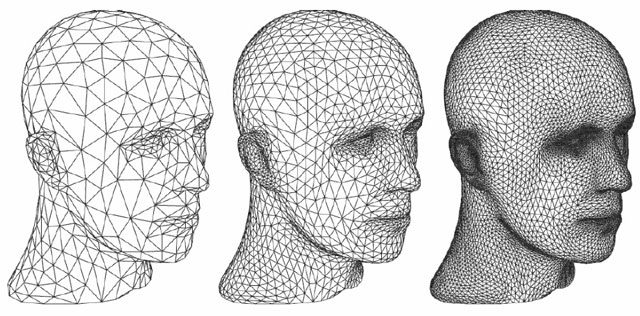
\includegraphics[width=0.7\textwidth]{geometryshader.jpg}
	\caption{Purpose of geometry shader.}
\end{figure}
The third stage is an optional geometry shader, this stage won't be covered in depth, but it is essentially in charge of creating additional geometry (extra vertices) on the fly (at runtime).\newline\par

\subsubsection{Rasterization stage}
The fourth stage is rasterization, this is where the algorithm gets it's name. The rasterizer is in charge of a not only rasterization, but also homogeneous divide, clipping, culling and viewport transform. \newline\par

\begin{minipage}{0.5\textwidth}
	\centering
	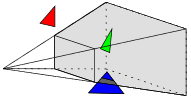
\includegraphics[width=\textwidth]{culling.png}
\end{minipage} \hfill
\begin{minipage}{0.5\textwidth}
	The first task of the rasterizer is primitive culling. The shapes that made it to the rasterizer are checked based on their normals. The normal of a primitive/vertex tells us if the face is facing away from us or not. This simple operation can be demonstrated using the dotproduct, however this does get handled by the specifications (e.g. DirectX/OpenGL) rasterizer. In it's essence the calculation will translate to if the dotproduct is negative then the face is facing away, if it's positive then it's facing toward us.
\end{minipage}

\pagebreak

\begin{minipage}{0.5\textwidth}
	The second task is the clipping stage, in this stage we clip triangles that lie (partly) outside of the view frustum. This effectively removes those triangles and prevents them from being projected/rendered. 
\end{minipage} \hfill
\begin{minipage}{0.5\textwidth}
	\centering
	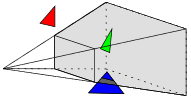
\includegraphics[width=0.8\textwidth]{clipping.png}
\end{minipage}

\vspace{0.5cm}

\begin{minipage}{0.4\textwidth}
	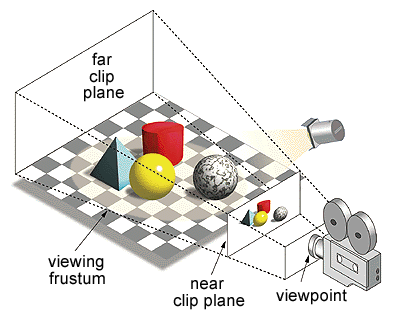
\includegraphics[width=\textwidth]{frustrum.png}
\end{minipage} \hfill
\begin{minipage}{0.59\textwidth}
	The third task of the rasterizer is the homogeneous divide. The previous stages were in charge of transforming the vertices from model space into clipping space, this is done by multiplying the world, view and projection matrix with the vertices this yields a valid projection but does not account for depth information (f.e. objects that are nearby will appear the same as objects from afar) this is where the z-component comes in, seeing the z stores our depth information. Before we apply the projectionmatrix we store the z-component as an additional w component.
\end{minipage}

\vspace{0.25cm}

The homogeneous divide is just a specific term for converting the homogeneous coordinate back to w=1 meaning we put the vertices in their normalized device coordinates (in the -1 to 1 range) effectively scaling all objects to their rightful dimensions.\newline\par

The fourth stage is the viewport transform. In the viewport transform we essentially translate all the vertex positions that are now in normalized device coordinates (NDC) and transform them to window space. These are then the coordinates that are being rasterized to the output image. This process is outlined in figure \ref{fig:coordinates} (part with green outline).

\vspace{0.5cm}

\begin{minipage}{0.4\textwidth}
	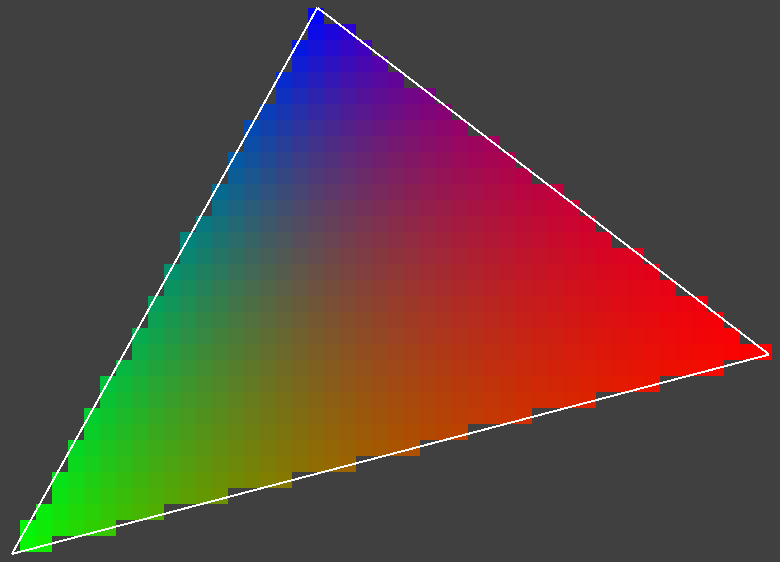
\includegraphics[width=0.95\textwidth]{pixelisation.png}
\end{minipage} \hfill
\begin{minipage}{0.59\textwidth}
	The final task pixelisation (rasterisation) is the process of converting continuous primitives into discrete pixel fragments. The rasterizer does so by interpolating between vertex attributes (data that vertex holds) like color, normals, texture coordinates and positions. It then stores that information in the pixel fragments before finally sending it off to the pixel/fragment shader to be shaded.
\end{minipage}

\pagebreak

\subsubsection{Fragment shader}
The fifth stage then applies shading to those pixel fragments.

\subsubsection{Test and blending stage}
Finally we've got the testing and blending stage.

\pagebreak

\section{Hybrid rendering approach}
\begin{figure}[h]
	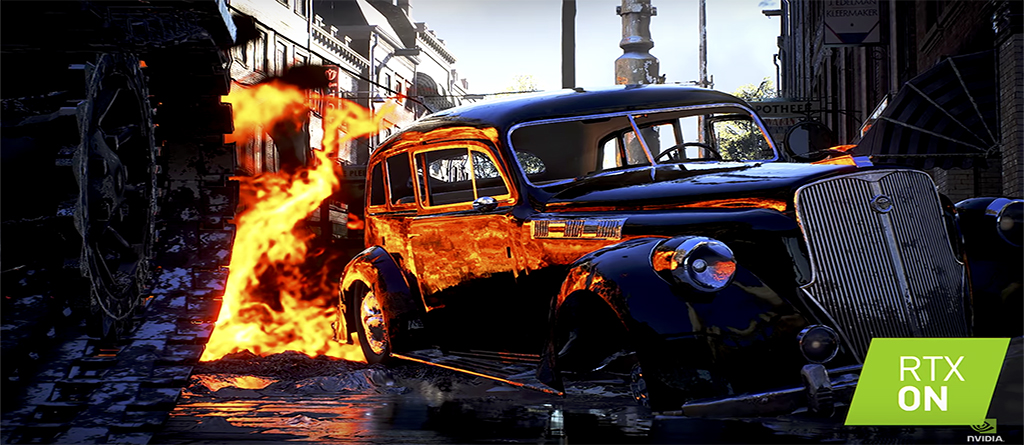
\includegraphics[width=\textwidth]{hybrid.jpg}
	\caption{Hybrid rendering empowered by Nvidia RTX}
\end{figure}
The different rendering techniques have been covered, now onto a hybrid solution where rasterization and raytracing are combined to achieve a new pipeline. Most hybrid approaches replace the first stage of ray-tracing, which is sending out our primary rays to retrieve surface information, by rasterization. This effectively reduces the amount of rays by half. Ray-tracing comes into play for sending out our reflected rays, which could be anything from sending out new primary rays to secondary (shadow) rays. This introduction of raytracing essentially brings us world information whereas normally you'd only have surface information. To be able to augment rasterization with raytracing we will need to postpone our lighting effects to a later stage. In a forward rendering pipeline the lighting is done per mesh in the fragment shader stage, effectively disabling us from hooking raytracing to that pipeline.

\pagebreak
\subsection{Raytracing in rasterization}

\subsubsection{Forward vs deferred rendering}
Lorem ipsum dolor sit amet, consectetur adipiscing elit. Duis risus ante, auctor et pulvinar non, posuere ac lacus. Praesent egestas nisi id metus rhoncus ac lobortis sem hendrerit. Etiam et sapien eget lectus interdum posuere sit amet ac urna. Aliquam pellentesque imperdiet erat, eget consectetur felis malesuada quis. Pellentesque sollicitudin, odio sed dapibus eleifend, magna sem luctus turpis, id aliquam felis dolor eu diam. Etiam ullamcorper, nunc a accumsan adipiscing, turpis odio bibendum erat, id convallis magna eros nec metus. Sed vel ligula justo, sit amet vestibulum dolor. Sed vitae augue sit amet magna ullamcorper suscipit. Quisque dictum ipsum a sapien egestas facilisis.

\subsubsection{Deferred shading}
Lorem ipsum dolor sit amet, consectetur adipiscing elit. Duis risus ante, auctor et pulvinar non, posuere ac lacus. Praesent egestas nisi id metus rhoncus ac lobortis sem hendrerit. Etiam et sapien eget lectus interdum posuere sit amet ac urna. Aliquam pellentesque imperdiet erat, eget consectetur felis malesuada quis. Pellentesque sollicitudin, odio sed dapibus eleifend, magna sem luctus turpis, id aliquam felis dolor eu diam. Etiam ullamcorper, nunc a accumsan adipiscing, turpis odio bibendum erat, id convallis magna eros nec metus. Sed vel ligula justo, sit amet vestibulum dolor. Sed vitae augue sit amet magna ullamcorper suscipit. Quisque dictum ipsum a sapien egestas facilisis.

\subsubsection{G-Buffers}
Lorem ipsum dolor sit amet, consectetur adipiscing elit. Duis risus ante, auctor et pulvinar non, posuere ac lacus. Praesent egestas nisi id metus rhoncus ac lobortis sem hendrerit. Etiam et sapien eget lectus interdum posuere sit amet ac urna. Aliquam pellentesque imperdiet erat, eget consectetur felis malesuada quis. Pellentesque sollicitudin, odio sed dapibus eleifend, magna sem luctus turpis, id aliquam felis dolor eu diam. Etiam ullamcorper, nunc a accumsan adipiscing, turpis odio bibendum erat, id convallis magna eros nec metus. Sed vel ligula justo, sit amet vestibulum dolor. Sed vitae augue sit amet magna ullamcorper suscipit. Quisque dictum ipsum a sapien egestas facilisis.

\subsection{Raytraced shadows}
\begin{wrapfigure}{r}{0.4\textwidth}
	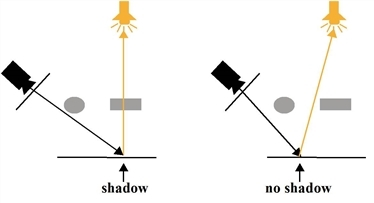
\includegraphics[width=0.4\textwidth]{shadows.jpg}
\end{wrapfigure}
For example when looking at ray-traced shadows. To determine if a pixel should be shaded or not a primary ray is cast from that pixel into the scene, material information is then gathered and additional secondary rays are being cast towards the relevant lights. If that secondary ray/shadow ray is occluded by another object then that pixel will be shaded using only the material information, if it isn't occluded however we can add the target lights information to to the shaders equation.\newline\par

\subsubsection{Soft shadows}
Test test test

\subsection{Optimizations}
Lorem ipsum dolor sit amet, consectetur adipiscing elit. Duis risus ante, auctor et pulvinar non, posuere ac lacus. Praesent egestas nisi id metus rhoncus ac lobortis sem hendrerit. Etiam et sapien eget lectus interdum posuere sit amet ac urna. Aliquam pellentesque imperdiet erat, eget consectetur felis malesuada quis. Pellentesque sollicitudin, odio sed dapibus eleifend, magna sem luctus turpis, id aliquam felis dolor eu diam.

%%%%%%%%%%%%%%%%
% NEW CHAPTER! %
%%%%%%%%%%%%%%%%
\chapter{Case study}
Lorem ipsum dolor sit amet, consectetur adipisicing elit, sed do eiusmod tempor incididunt ut labore et dolore magna aliqua. Ut enim ad minim veniam, quis nostrud exercitation ullamco laboris nisi ut aliquip ex ea commodo consequat.

\section{Implementation rasterization}
\subsection{Window creation}
\subsection{Rendering specification}
\subsection{Shader loading}
\subsection{Coordinate systems}
\subsection{Model loading}
\subsection{Texture loading}
\subsection{Deferred shading}
\section{Implementation ray-tracing}
\subsection{Radeon rays implementation}
\subsection{Shadow implementation}
\subsection{Optimizations}

\chapter{Conlusion}
Lorem ipsum dolor sit amet, consectetur adipisicing elit, sed do eiusmod tempor incididunt ut labore et dolore magna aliqua. Ut enim ad minim veniam, quis nostrud exercitation ullamco laboris nisi ut aliquip ex ea commodo consequat.

\bibliographystyle{}
\bibliography{}
\begin{thebibliography}{Xyz12}
	
	\bibitem{voica14}
	Alexandru Voica,
	2014,
	Practical techniques for ray tracing in games,
	\url{http://www.gamasutra.com/blogs/AlexandruVoica/20140318/213148/Practical_techniques_for_ray_tracing_in_games.php}
	
	\bibitem{voica15}
	Alexandru Voica,
	2015,
	Ray tracing made easy,
	\url{http://www.alexvoica.com/ray-tracing-made-easy/#sthash.q1sHqqiT.dpbs}
	
	\bibitem{einig17}
	Mathieu Einig,
	2017,
	Hybrid rendering for real-time lighting: ray tracing vs rasterization,
	\url{https://www.imgtec.com/blog/hybrid-rendering-for-real-time-lighting/}
	
	\bibitem{caulfield18}
	Brian Caulfield,
	2018,
	What's the difference between ray tracing and rasterization?,
	\url{https://blogs.nvidia.com/blog/2018/03/19/whats-difference-between-ray-tracing-rasterization/}
	
	\bibitem{pipeline18}
	Wikipedia,
	2018,
	Graphics pipeline,
	\url{https://en.wikipedia.org/wiki/Graphics_pipeline}
	
	\bibitem{scratchapixel18}
	Scratchapixel,
	2018,
	Ray-Tracing: Generating Camera Rays,
	\url{https://www.scratchapixel.com/lessons/3d-basic-rendering/ray-tracing-generating-camera-rays}
\end{thebibliography}

%%%%%%%%%%%%%%%%
% NEW CHAPTER! %
%%%%%%%%%%%%%%%%
\chapter*{Appendices}

\end{document}
